% Template taken with permission from Richard Hu
% Modified by Rahul Shah
% Last Updated: 2021-01-29 22:15

\documentclass[11pt]{article}
\usepackage{header}
\usepackage{mathrsfs}
\usepackage{mdframed}
\usepackage{pdfpages}
\usepackage{titlesec}

\newmdenv[%
    leftmargin=-5pt,
    rightmargin=-5pt, 
    innerleftmargin=5pt,
    innerrightmargin=5pt,
    backgroundcolor=brown!10,
]{Answer}%
\def\title{Homework 02}

\def\R{\mathbb{R}} % Real Numbers
\def\P{\mathbb{P}}
\newcommand{\pd}[2]{\frac{\partial{#1}}{\partial{#2}}}
\let\originalmiddle=\middle
\def\middle#1{\mathrel{}\originalmiddle#1\mathrel{}}
\newcommand\aug{\fboxsep=-\fboxrule\!\!\!\fbox{\strut}\!\!\!}


\makeatletter
\newcount\my@repeat@count
\newcommand{\myrepeat}[2]{%
  \begingroup
  \my@repeat@count=\z@
  \@whilenum\my@repeat@count<#1\do{#2\advance\my@repeat@count\@ne}%
  \endgroup
}
\makeatother

\titlelabel{\thetitle.\enspace}


\begin{document}
\maketitle
\fontsize{12}{15}\selectfont

\begin{center}
    HW Due: February 5, 2021, at 23:59 \\
    Self-grades due: February 8, 2021, at 23:59
\end{center}


\section{Reading Assignment}

    For this homework, please review Note 1B and read Note 2A. They will provide an overview of Gaussian elimination, vectors, and matrices. You are always welcome and encouraged to read beyond this as well, in particular, a quick look at Note 3 will help you. 
    \begin{itemize}
        \item Describe how Gaussian elimination can help you understand if there are no solutions to a particular system of equations? 
        \item What about a unique solution?
        \item Does a row of zeros always mean there are infinite solutions?
    \end{itemize}

    \begin{Answer}
        Your answer goes here.
        \begin{itemize}
            \item \myrepeat{10}{This is a bunch of filler text which you should delete. }
            \item \myrepeat{10}{This is a bunch of filler text which you should delete. }
            \item \myrepeat{10}{This is a bunch of filler text which you should delete. }
        \end{itemize}
    \end{Answer}

\newpage


\section{Gaussian Elimination}

    (a) In this problem we will investigate the relationship between Gaussian elimination and the geometric interpretation of linear equations. You are welcome to draw plots by hand or using software. Please be sure to label your equations with a legend on the plot
    
    \begin{enumerate}[i.]
        \item Draw the following set of linear equations in the x-y plane. If the lines intersect, write down the point or points of intersection.
        
            \begin{equation}
                x+2y = 4
            \end{equation}
            \begin{equation}
                2x-4y = 4
            \end{equation}
            \begin{equation}
                3x-2y = 8
            \end{equation}
        
        \item Write the above set of linear equations in augmented matrix form and do the first step of Gaussian elimination to eliminate the $x$ variable from equation 2. Now, the second row of the augmented matrix has changed. Plot the corresponding new equation created in this step on the same graph as above. What do you notice about the new line you draw?
        \item Complete all of the steps of Gaussian elimination including back substitution. Now plot the new equations represented by the rows of the augmented matrix in the last step (after completing back substitution) on the same graph as above. What do you notice about the new line you drew?
    \end{enumerate}

    \begin{Answer}
        Your answer goes here.
        \begin{itemize}
            \item \myrepeat{10}{This is a bunch of filler text which you should delete. }
            \item \myrepeat{10}{This is a bunch of filler text which you should delete. }
        \end{itemize}
    \end{Answer}

\newpage

    (b) Write the following set of linear equations in augmented matrix form and use Gaussian elimination to determine if there are no solutions, infinite solutions, or a unique solution. If any solutions exist, determine what they are. You may do this problem by hand or use a computer. We encourage you to try it by hand to ensure you understand Gaussian elimination.
    
    \[x+2y+5z = 3\]
    \[x+12y+6z = 1\]
    \[2y+z = 4\]
    \[3x+16y+16z = 7\]

    \begin{Answer}
        Your answer goes here.
        
        \par
        
        \myrepeat{35}{This is a bunch of filler text which you should delete. }
    \end{Answer}

\newpage

    (c) Consider the following system of equations:
    
    \[
        x+2y+5z = 6
    \]
    \[
        3x+9y+6z = 3
    \]
    
    You are given a set S of candidate solutions,
    
    \[
        S=\left \{\vec{v} \,\middle|\, 
        \vec{v} = \begin{bmatrix}
                    x \\
                    y \\
                    z \\
                \end{bmatrix} 
                =
                \begin{bmatrix}
                    16 \\
                    -5 \\
                     0 \\
                \end{bmatrix} 
                +
                \begin{bmatrix}
                  -11 \\
                    3 \\
                    1 \\
                \end{bmatrix} t
                ,  \ 
                t \in \R
        \right \}
    \]
    
    This vector notation can be expressed in terms of its components:
    
    \begin{center}
        
        $
            \vec{v} = \begin{bmatrix}
                    16 - 11t \\
                    -5 +  3t \\
                           t \\
                 \end{bmatrix}    
        $     
        means   
        $
            \begin{aligned}
                x &= 16 - 11t \\
                y &= -5 +  3t \\
                z &= t
            \end{aligned}
        $
    \end{center}
    Show, by substitution, that any $\vec{v} \in S$ is a solution to the system of equations given above. Note that this means that the candidate solution must satisfy the system of equations for all $t \in \R$.

    \begin{Answer}
        Your answer goes here.
        
        \par
        
        \myrepeat{25}{This is a bunch of filler text which you should delete. }
    \end{Answer}

\newpage

    (d) Consider the following system:
    
    \[
        4x+4y+4z+w+v = 1
    \]
    \[
        x+y+2z+4w+v = 2
    \]
    \[
        5x+5y+5z+w+v = 0
    \]
    
    If you were to write the above equations in augmented matrix form and use Gaussian elimination to solve the system, you would get the following (for extra practice, you can try and do this yourself):
    
    $$
    \begin{bmatrix}
        1 & 1 & 0 & 0 & 3  &\aug& 16\hfill \\
        0 & 0 & 1 & 0 & -3 &\aug& -17\hfill \\
        0 & 0 & 0 & 1 & 1  &\aug& 5
    \end{bmatrix}
    $$
    
    How many variables are free variables? Determine the solutions to the set of equations.

    \begin{Answer}
        Your answer goes here.
        
        \par
        
        \myrepeat{25}{This is a bunch of filler text which you should delete. }
    \end{Answer}

\newpage

\section{Linear Dependence}

    State if the following sets of vectors are linearly independent or dependent. If the set is linearly dependent, provide a linear combination of the vectors that sum to the zero vector.
    
    \vspace{5mm}
    
    (a) 
        $
            \left \{
                \begin{bmatrix}
                    -5 \\
                     2
                \end{bmatrix},
                \begin{bmatrix}
                    5 \\
                    2
                \end{bmatrix}
            \right \}
        $

    \vspace{5mm}

    \begin{Answer}
        Your answer goes here.
        
        \par
        
        \myrepeat{30}{This is a bunch of filler text which you should delete. }
    \end{Answer}

\newpage

    
    (b) 
        $
            \left \{
                \begin{bmatrix}
                    -1 \\
                     1 \\
                     0 \\
                    -1 \\
                    1
                \end{bmatrix},
                \begin{bmatrix}
                    1 \\
                    2 \\
                    3 \\
                   -2 \\
                   -1
                \end{bmatrix},
                \begin{bmatrix}
                   -1 \\
                    0 \\
                   -1 \\
                    0 \\
                    1
                \end{bmatrix}
            \right \}
        $

    \vspace{5mm}

    \begin{Answer}
        Your answer goes here.
        
        \par
        
        \myrepeat{30}{This is a bunch of filler text which you should delete. }
    \end{Answer}

\newpage

    
    (c) 
        $
            \left \{
                \begin{bmatrix}
                     2 \\
                     2 \\
                     0
                \end{bmatrix},
                \begin{bmatrix}
                    0 \\
                    1 \\
                    1
                \end{bmatrix},
                \begin{bmatrix}
                    2 \\
                    4 \\
                   -1
                \end{bmatrix},
                \begin{bmatrix}
                    0 \\
                   -1 \\
                    1
                \end{bmatrix}
            \right \}
        $

    \vspace{5mm}

    \begin{Answer}
        Your answer goes here.
        
        \par
        
        \myrepeat{30}{This is a bunch of filler text which you should delete. }
    \end{Answer}

\newpage

    
    (d) 
        $
            \left \{
                \begin{bmatrix}
                     1 \\
                     1 \\
                     1 \\
                     0 \\
                     0
                \end{bmatrix},
                \begin{bmatrix}
                     1 \\
                     1 \\
                    -2 \\
                     2 \\
                     0
                \end{bmatrix},
                \begin{bmatrix}
                     0 \\
                     0 \\
                     0 \\
                     0 \\
                     0
                \end{bmatrix}
            \right \}
        $

    \vspace{5mm}

    \begin{Answer}
        Your answer goes here.
        
        \par
        
        \myrepeat{30}{This is a bunch of filler text which you should delete. }
    \end{Answer}

\newpage

\section{Filtering Out The Troll}

    TLDR: A troll interfered with a meeting you recorded. You remembered the locations of the speaker and the troll and created the diagram shown in Figure 1. You are located at the origin.
    
    \begin{figure}[h]
        \centering
        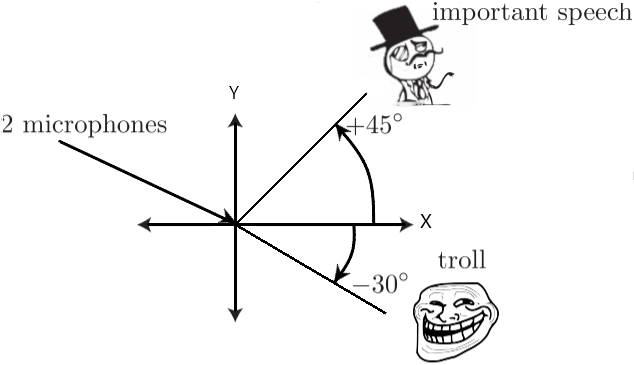
\includegraphics[scale=0.25]{troll}
        \caption{ Locations of the speaker and the troll.}
    \end{figure}
    
    Signals are recorded differently by microphones based on their angles of arrival. The first microphone weights (multiplies) a signal, coming from an angle $\theta$ with respect to the x-axis, by the factor $f_1(\theta) = \cos(\theta)$. If two signals are simultaneously playing (as is the case with the speech and the troll interference), then a linear combination (i.e. a weighted sum) of both the signals is recorded, each weighted by the respective $f_1(\theta)$ for their angles. The second microphone weights a signal, coming from an angle $\theta$ with respect to the x-axis, by the factor $f_2(\theta) = \sin(\theta)$.
    \par
    For example, an audio source that lies on the x axis will be recorded by the first microphone with weight equal to 1 (since $\cos(0) = 1$), but will not be recorded up by the second microphone (since $\sin(0) = 0$). Note that the weights can also be negative.
    \par
    Let us represent the speech sample at a particular time-instant by the variable a and the interference caused by the troll at the same time-instant by the variable b. Remember, we do not know either a or b. The recording of the first microphone at that time instant is given by $m_1 = f_1(\alpha) \cdot a + f_1(\beta) \cdot b$ and $m_2 = f_2(\alpha) \cdot a + f_2(\beta) \cdot b$ where $\alpha$ and $\beta$ are the angles at which the public speaker $A$ and the troll $B$ respectively are located with respect to the x-axis, and variables a and b are the audio signals produced by the public speaker $A$ and the troll $B$ respectively.
    
    (a) Plug in the values of $\alpha$ and $\beta$ to write the recordings of the two microphones $m_1$ and $m_2$ as a linear combination (i.e. a weighted sum) of $a$ and $b$.
    \begin{Answer}
        Your answer goes here.
    \end{Answer}


\newpage

    (b) Solve the system you wrote out on the earlier part to recover the important speech $a$, as a weighted combination of $m_1$ and $m_2$. In other words, write $a = u\cdot m_1 + v \cdot m_2$ (where $u$ and $v$ are scalars). What are the values of $u$ and $v$?

    \begin{Answer}
        Your answer goes here.
        
        \par
        
        \myrepeat{50}{This is a bunch of filler text which you should delete. }
    \end{Answer}

    % TODO: upload your own my_ipyntbk.pdf 
    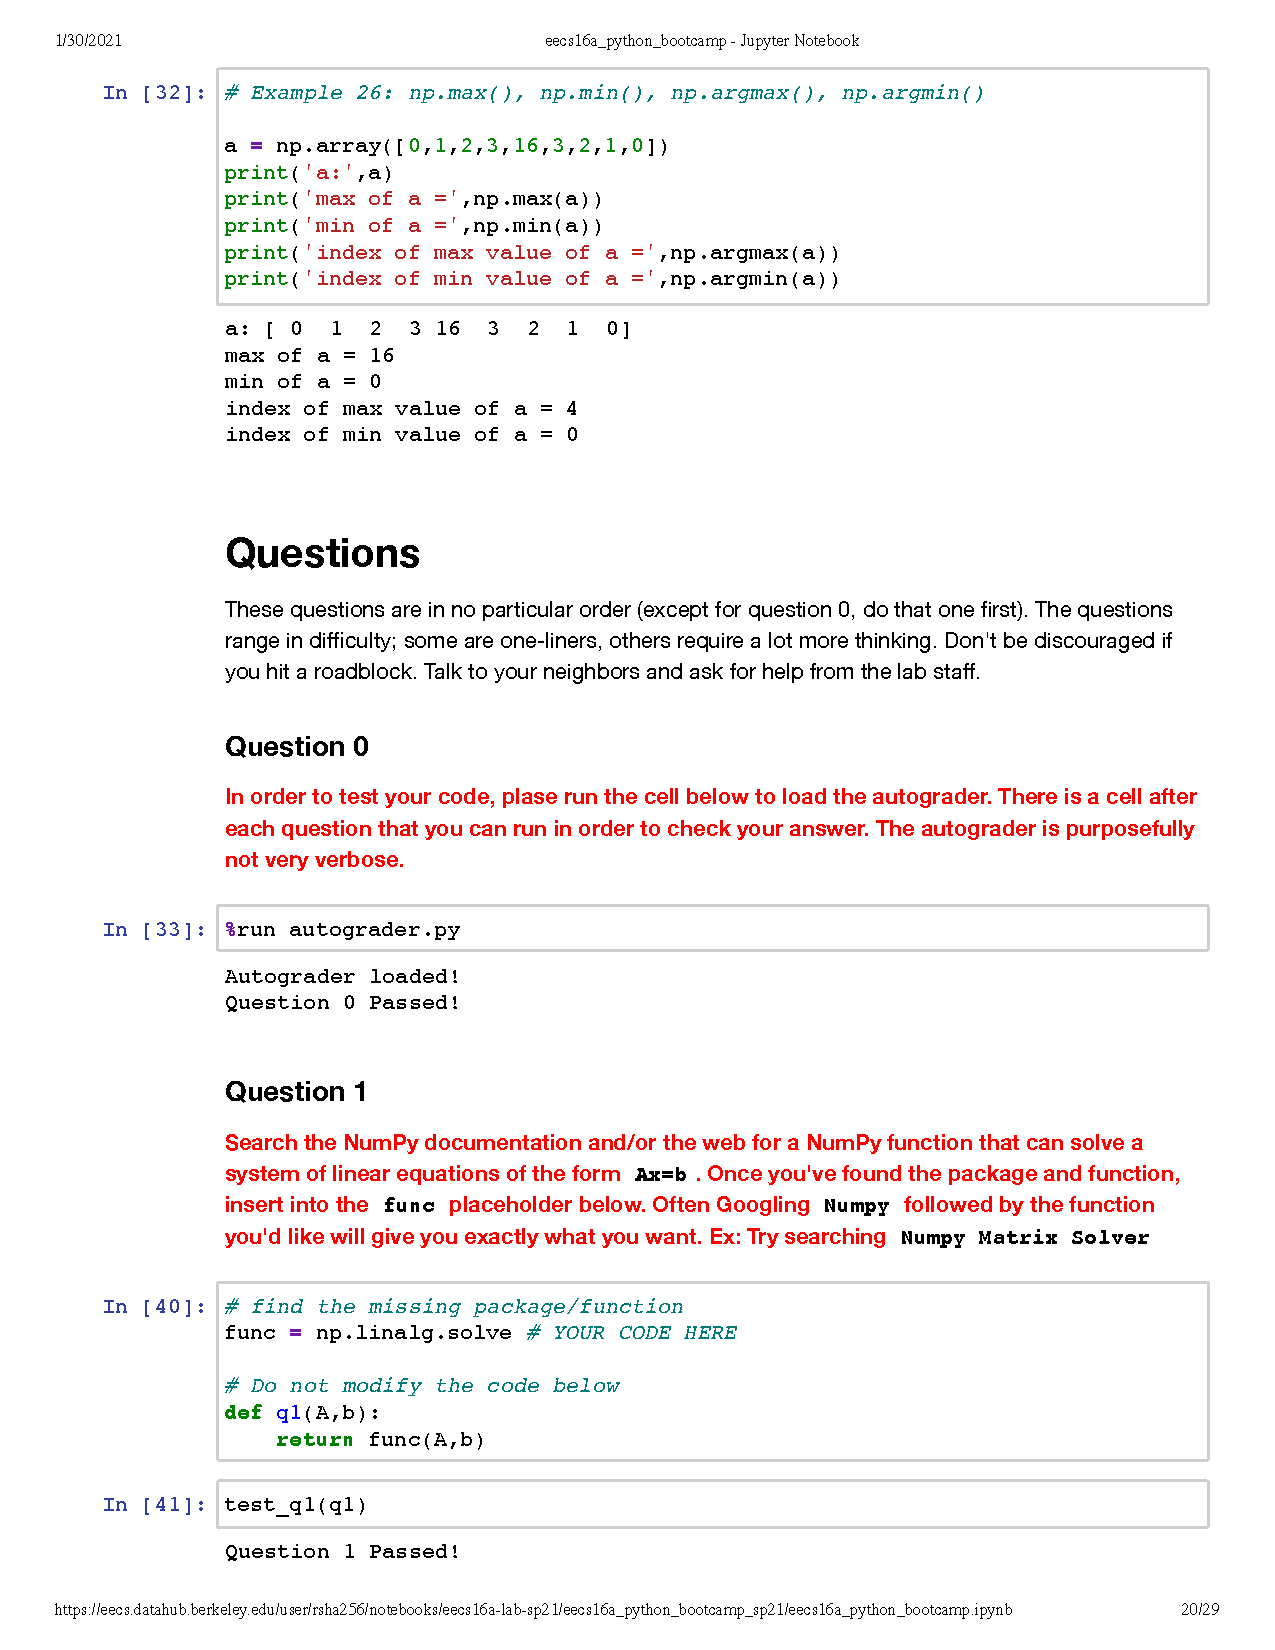
\includepdf[pages=-, noautoscale=true, scale=.8]{my_ipyntbk.pdf} 

\newpage

\section*{6. Fountain Codes}

    Alice wants to send a message to her friend Bob. Alice sends her message $\vec m$ across a wireless channel in the form of a transmission vector $\vec w$. Bob receives a vector of symbols denoted as $\vec r$. Alice knows some of the symbols in the transmission vector that she sends may be corrupted, so she needs
    a way to protect her message from the corruptions.
    \par
    One way to accomplish this goal is to use fountain codes, a type of error correcting code. The basic principle is that instead of sending the exact message, Alice sends a modified longer version of the message so that even if some parts are corrupted Bob can recover what she meant.
    
    The message that Alice wants to send to Bob is the three numbers $a$, $b$, and $c$. The message vector representing these numbers is 
    $
        \vec m = \begin{psmallmatrix}
                    a \\
                    b \\
                    c
                \end{psmallmatrix}
    $. Figure 2 shows how Alice’s message is encoded in a transmission vector and how Bob’s received vector may have some corrupted symbols.
    \begin{figure}[h]
        \centering
        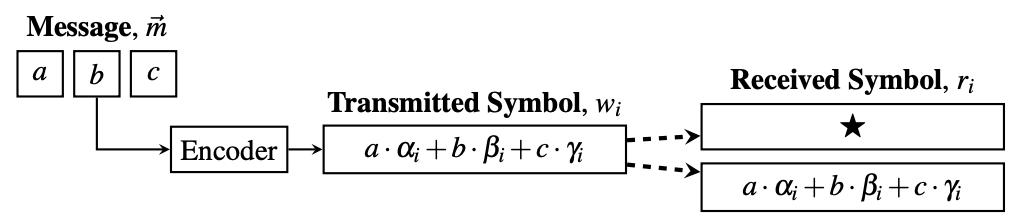
\includegraphics[scale=0.25]{encoder}
        \caption{Each symbol in a transmission vector $\vec w$ is a linear combination of $a$, $b$, and $c$. Each transmitted symbol, $w_i$, is either received exactly as it was sent, or it is corrupted. A corrupted symbol is denoted by $\star$. The $i$th row of a symbol generating matrix $G$ determines the values of $\alpha_i$, $\beta_i$, $\gamma_i$.}
    \end{figure}
    
    (a) Since Alice has three numbers she wishes to send, she could transmit six symbols in her transmission vector for redundancy. This transmission strategy is called the “repetition code”.
    
    If Alice uses the repetition code, her transmission vector is $\vec w =
                                                                    \begin{psmallmatrix}
                                                                    a \\
                                                                    b \\
                                                                    c \\
                                                                    a \\
                                                                    b \\
                                                                    c
                                                                    \end{psmallmatrix}
                                                                  $.
    As depicted in Figure 2, the received vector may have corrupted symbols. For example, suppose only the first symbol was corrupted, then Bob would receive the vector $\vec r =
                    \begin{psmallmatrix}
                        \star \\
                            b \\
                            c \\
                            a \\
                            b \\
                            c
                    \end{psmallmatrix}
            $ where the $\star$ symbol represents a corrupted symbol. Using the repetition code scheme, give an example of a received vector $\vec r$ with only two corrupted symbols such that $a$ is unrecoverable but $b$ and $c$ are still recoverable.
    \begin{Answer}
        Answer goes here, $\vec r =
                    \begin{bmatrix}
                        69 \\
                        420 \\
                        \ldots
                    \end{bmatrix}
            $
    \end{Answer}


\newpage

(b) Alice can generate $\vec w$ by multiplying her message $\vec m$ by a matrix. Write a matrix-vector multiplication that Alice can use to generate $\vec w$ according to the repetition code scheme. Specifically, find a “generating” matrix $G_R \text{ s.t. } G_R \vec m = \vec w$, where $\vec w = \begin{bmatrix}
                                                a \\
                                                b \\
                                                c \\
                                                a \\
                                                b \\
                                                c
                                            \end{bmatrix}                       
                                    $.

    \vspace{5mm}

    \begin{Answer}
        Your answer goes here.
        
        \par
        
        \myrepeat{30}{This is a bunch of filler text which you should delete. }
    \end{Answer}

\newpage

    (c) Instead of a repetition code, it is also possible to use codes like fountain codes. Alice and Bob can choose any symbol generating matrix, as long as they agree upon it in advance. Each matrix represents a "code." Alice’s TA recommends using the symbol generating matrix $G_F$: 
        \[
            G_F = \begin{bmatrix}
                1 & 0 & 0 \\
                0 & 1 & 0 \\
                0 & 0 & 1 \\
                1 & 1 & 0 \\
                1 & 0 & 1 \\
                0 & 1 & 1 \\
                1 & 1 & 1
                \end{bmatrix}.
        \]
    Alice then uses the symbol generating matrix $G_F$ to produce a new transmission vector: $G_R \vec m = \vec w$.
    Suppose Bob receives the vector $\vec r = \begin{bmatrix}
                                                7     \\
                                                \star \\
                                                \star \\
                                                3     \\
                                                4     \\
                                                \star \\
                                                \star
                                              \end{bmatrix}
                                    $, which is a corrupted version of $\vec w$.
    Write a system of linear equations that Bob can use to recover the message vector $\vec m$. Solve it to recover
    the three numbers that Alice sent.
    \\
    $\textbf{Hint: }$ Consider the rows of $G_F$ that correspond to the uncorrupted symbols in $\vec r$.
    
        \vspace{5mm}
    
        \begin{Answer}
            Your answer goes here.
            
            \par
            
            \myrepeat{30}{This is a bunch of filler text which you should delete. }
        \end{Answer}
    
    \newpage


    (d) We explore one example case where Alice and Bob agree to use $G_F$ (i.e. $G_F\vec m =\vec w$) and there are three corruptions, so Bob receives four uncorrupted symbols.
    Suppose Bob receives $\vec r =
                                \begin{bmatrix}
                                    1     \\
                                    \star \\
                                    3     \\
                                    \star \\
                                    4     \\
                                    \star \\
                                    9
                                \end{bmatrix}
                         $. Can you determine the message $\vec m$ that Alice sent?
    \\
    $\textbf{Note: }$ it can be shown that receiving $\textit{any}$ four uncorrupted symbols when Alice is using $G_F$ is enough to recover Alice’s message. On the other hand, we showed in part (a) that receiving $\textit{any}$ four uncorrupted symbols using $G_R$ does not guarantee we can recover Alice’s message. This is why, in practice, we would prefer to use the fountain code $G_F$ instead of the repetition code $G_R$ — it is a more reliable way to send messages.
    
    \begin{Answer}
        Your answer goes here.
        \myrepeat{20}{This is a bunch of filler text which you should delete. }
    \end{Answer}

\newpage


\section*{7. Show It!}
    (a) $\textbf{Show that if the system of linear equations, A}\vec x =\vec b,\textbf{ has infinitely many solutions,}$
    
    $\textbf{then columns of A are linearly dependent.}$
    
    \begin{enumerate}[(i)]
        \item $\textbf{First Step: Write what you know:}$
        Think about the $\textbf{information we already know}$ from the problem statement. We know that system of equations, $A\vec x =\vec b$, has infinitely many solutions. Infinitely many solutions are hard to work with, but perhaps we can simplify to something that we can work with. If the system has infinite number of solutions, it must have at least \_\_\_ distinct solutions % TODO: (Fill in the blank).
        \par
        So let us assume that $\vec u$ and $\vec v$ are two different vectors, both of which are solutions to $A\vec x =\vec b$.
        Express the sentence above in a mathematical form (Just writing the equations will suffice; no need to do further mathematical manipulation).
        \item $\textbf{Second Step: What we want to show:}$
            We $WTS$ that the columns of $\textbf A$ are linearly dependent. Let us assume that $\textbf A$ has columns $\vec c_1, \vec c_2, ..., \text{ and } \vec  c_n, \text{s.t. } \textbf A = \begin{bmatrix}
                                            \vec c_1 & \vec c_2 & \vec  c_n
                                          \end{bmatrix}
                                                $. Using the
            definition of linear dependence from Note 3 Subsection 3.1.1, write a mathematical equation that conveys linear dependence of $\vec c_1, \vec c_2, ..., \text{ and } \vec  c_n$.
        \item $\textbf{Third Step: Manipulating what we know:}$
        Since your answer to (ii) is expressed in terms of the column vectors of A, let us try to express the mathematical equations from (i), in terms of the column vectors too. For example, we can write
        \[
            \textbf A\vec x =\vec b
        \]
        \[
            \implies
            \begin{bmatrix}
                \vec c_1 & \vec c_2 & \ldots & \vec  c_n
            \end{bmatrix}
            \begin{bmatrix}
                x_1 \\
                x_2 \\
                \ldots \\
                x_n
            \end{bmatrix}
        \]
        \[
            \implies
            x_1\vec c_1 + x_2\vec c_2 + \ldots + x_n\vec c_n = \vec b
        \]
        Notice that $x_1, \ldots x_n$ etc are scalars. Now use your answer to part (i) to repeat the above formulation for distinct solutions $\vec u$ and $\vec v$.
        \item $\textbf{Fourth Step: Connecting it up:}$
        Now think about how you can mathematically manipulate your answer from part (iii) (Manipulating what we know) to match the pattern of your answer from part (ii) (What we want to show).
    \end{enumerate}
    \begin{Answer}
        answer
    \end{Answer}

\newpage

    
    (b) Now try this proof on your own. Similar proofs will also be covered in your discussion section 2A.
    Given some set of vectors $\{\vec v_1, \vec v_2,\ldots,\vec v_n\},$ show the following:
    \[
        \text{span}\{\vec v_1,\vec v_2,\ldots,\vec v_n\} = \text{span}\{\vec v_1 +\vec v_2,\vec v_2,\ldots,\vec v_n\}
    \]
    In other words, we can replace one vector with the sum of itself and another vector and not change their span.
    \\
    In order to show this, you have to prove the two following statements:
    \begin{enumerate}
        \item If a vector $\vec q$ belongs in span$\{\vec v_1, \vec v_2, \ldots , \vec v_n\}$, then it must also belong in span$\{\vec v_1 +\vec v_2,\vec v_2,\ldots,\vec v_n\}$.
        \item If a vector~r belongs in span$\{\vec v_1 +\vec v_2,\vec v_2,\ldots,\vec v_n\}$, then it must also belong in span$\{\vec v_1, \vec v_2, \ldots , \vec v_n\}$.
    \end{enumerate}
    In summary, you have to prove the problem statement from both directions.
    \begin{Answer}
        Your answer goes here.
        \begin{itemize}
            \item \myrepeat{20}{This is a bunch of filler text which you should delete. }
            \item \myrepeat{20}{This is a bunch of filler text which you should delete. }
        \end{itemize}
    \end{Answer}
\newpage

    (c) Let $n$ be a positive integer. Let $\{\vec v_1, \vec v_2, \ldots , \vec v_k\}$ be a set of k linearly dependent vectors in $\R^n$. Show that for $any \ n\times n$ matrix $\textbf A$, the set $\{\textbf A~\vec v_1, \textbf A~\vec v_2,\ldots , \textbf A~\vec v_k\}$ is a set of linearly dependent vectors.

    \begin{Answer}
        Your answer goes here.
        \myrepeat{50}{This is a bunch of filler text which you should delete. }
    \end{Answer}

\newpage

\section*{8. Homework Process and Study Group}

Who did you work with on this homework? List names and student ID’s. (In case you met people at homework party or in office hours, you can also just describe the group.) How did you work on this homework? If you worked in your study group, explain what role each student played for the meetings this week.

\begin{Answer}
    
\end{Answer}

\newpage

\end{document}